\documentclass[10pt]{article}
\usepackage[margin=0.82in]{geometry}
\usepackage{booktabs}
\usepackage{graphicx}
\usepackage{hyperref}
\usepackage{xcolor}

\title{Heterogeneous Reflex Reasoning:\\Where Multi-Engine Interface Knowledge Breaks}
\author{Working Draft}
\date{August 2026}

\begin{document}
\maketitle

\begin{abstract}
Where should knowledge of a deterministic execution interface live: in context,
in model weights, or in the runtime?  We test one bounded protocol spanning five
local engines---calculator, Datalog, ISA graph, date arithmetic, and dimensional
unit conversion---on Qwen3-0.6B, SmolLM2-1.7B, and Gemma3-1B.  A frozen benchmark
contains 200 training, 50 development, and 100 test rows, with 16 test tasks per
engine and 20 no-execution controls.  A prompt-derived deterministic reflex and
an oracle both execute the frozen forms exactly.  The learned policy does not:
at five engines, Qwen, SmolLM2, and Gemma reach engine-selection rates of 0.188,
0.350, and 0.000, respectively, and runtime-exact rates of 0.188, 0.313, and
0.000.  All preserve zero false activations, but every exact result sent through
the Qwen or SmolLM2 result-use pass is overridden.  In-context demonstrations
recover some engine families but grow from 39 to 118 static lexical interface
tokens and reach false-activation rates of 0.9--1.0 at several catalog sizes.
Textual schemas remain safe but inert.  A follow-up factorization adds 2,250
train, 450 development, and 900 test rows.  Its oracle-engine deterministic
parser is exact.  A benchmark-specific lexical router reaches 0.900 engine
selection and runtime exactness with zero false activation, whereas semantic
rules select 0.800 but execute 1.000 by substituting graph closure for Datalog,
and learned CPU routers select only 0.588 with 0.400 false activation.  Thus
exact execution and parsing belong in the runtime, but broad semantic selection
and result use remain unresolved.  The Paper 3 gate remains \texttt{no\_go}.
\end{abstract}

\section{Question and decision rule}

Paper 1 established a narrow placement rule for one calculator interface:
stable selection and serialization may live in adapter weights, while parsing,
bounds, execution, provenance, reinjection, and enforcement remain deterministic.
This paper asks whether that rule survives heterogeneous interfaces.  The central
question is:

\begin{quote}
Can one small model learn when to offload, select among five local engines,
serialize a bounded typed request, and preserve the exact result without prompt
cost growing with the engine catalog?
\end{quote}

The confirmatory gate is intentionally stronger than demonstrating that the
engines work.  At five engines, at least two model families must reach both
engine-selection and runtime-exact rates of at least 0.8, with false activation
at most 0.1.  Deterministic or oracle success cannot open this gate.

\section{Bounded heterogeneous runtime}

\subsection{Common envelope and registry}

All engines use one fail-closed registry and normalize into shared typed request,
result, and append-only state records.  The runtime
accepts exactly one complete fenced block from an enabled family.  Open fences,
multiple blocks, unknown engines, invalid dimensions, malformed payloads, and
over-budget state fail without execution.

The five block families are:

\begin{verbatim}
```calculator                 ```date
15246377 * 746647383          add 2026-08-28 P90D
```                           ```

```datalog                    ```units
fact link(a,b)                convert 7.3 mile -> kilometer
fact link(b,c)                ```
query reachable(a,c)
```

```graph
isa penguin bird
isa bird animal
query isa penguin animal
```
\end{verbatim}

The calculator is bounded and exact; Datalog uses finite forward chaining; the
graph engine computes bounded ISA closure and frame inheritance; date arithmetic
uses ISO dates and integer day durations; unit conversion rejects dimensional
mismatch.  No generated code, shell command, network action, general planner, or
unbounded theorem proving is permitted.

\subsection{Runtime reflex versus oracle}

The \emph{runtime reflex} recognizes only the five anchored natural-language
templates frozen by the benchmark and translates their captured fields into a
typed block.  Unknown or modified input returns no execution.  It does not read
the gold target.  The separate \emph{oracle} condition replays the gold typed
envelope.  Both are deterministic protocol validations, not model evidence and
not claims of open-ended semantic routing.

\section{Experimental design}

\subsection{Frozen data and leakage audit}

Table~\ref{tab:data} summarizes the benchmark.  Train, development, and test use
disjoint operand ranges, entity prefixes, dates, values, and control labels.  A
machine-readable audit finds no train/development/test signature overlap and no
answer string in a typed training target.  Targets teach requests, never engine
answers.

\begin{table}[ht]
\centering
\caption{Frozen benchmark composition.}
\label{tab:data}
\begin{tabular}{lrrr}
\toprule
Family & Train & Dev & Test \\
\midrule
Calculator & 32 & 8 & 16 \\
Datalog & 32 & 8 & 16 \\
ISA graph & 32 & 8 & 16 \\
Date/time & 32 & 8 & 16 \\
Units & 32 & 8 & 16 \\
No-execution control & 40 & 10 & 20 \\
\midrule
Total & 200 & 50 & 100 \\
\bottomrule
\end{tabular}
\end{table}

Nested catalogs contain 1, 2, 3, and 5 engines in the order calculator,
Datalog, graph, date, and units.  Each catalog includes all 20 controls.  This
changes the positive-task denominator (16, 32, 48, and 80) while holding the
control set fixed.

\subsection{Placement conditions}

We compare seven roles:

\begin{enumerate}
\item unassisted base-model exact answers;
\item context/ICL with one demonstration per enabled engine;
\item explicit textual schemas, because these checkpoints do not provide one
      uniform reliable native-tool interface;
\item one five-family rank-8 LoRA adapter plus a 26-token stable contract;
\item the anchored deterministic runtime reflex;
\item learned-policy plus deterministic validation/execution;
\item oracle typed-envelope replay.
\end{enumerate}

ICL and explicit-schema generation are tested on Qwen across all four catalog
sizes.  Learned-weight scaling uses the same five-family Qwen adapter while the
runtime enables nested catalogs.  Five-engine learned replication includes all
three model families.  Result use is assessed in the full five-engine adapter
runs; scaling sweeps stop after execution to avoid conflating selection with a
second generation pass.

\subsection{Adapters and XPU execution}

Each adapter trains for two epochs on the same 200 request-policy rows, with 50
development rows, rank 8, alpha 16, dropout 0.05, batch size 1, gradient
accumulation 8, learning rate $2\times10^{-4}$, and projections
\texttt{q/k/v/o}.  Final development losses are 0.00380 (Qwen), 0.00564
(SmolLM2), and 0.01122 (Gemma).  Low teacher-forced loss is therefore not treated
as evidence of held-out generation reliability.

All checkpoint revisions are pinned: Qwen \texttt{c1899de}, SmolLM2
\texttt{31b70e2}, and Gemma \texttt{dcc83ea}.  Training and generation use
PyTorch 2.13.0+XPU on Intel Graphics.  Interface generations have a 72-token cap;
the uniformly short unassisted exact-answer controls use a 24-token cap.

\subsection{Factorized scoring}

For positive rows we score DETECT, ENGINE SELECT, PAYLOAD NORMALIZE, EXECUTE,
runtime exactness, REINJECT, USE, and FINAL independently.  False activation is
defined only on controls.  USE, ignored-result, override, and wrong-
reinterpretation rates are conditioned on rows for which result use was actually
assessed.  Aggregate final accuracy includes controls and is reported only with
that caveat.  Costs include static lexical interface tokens, model tokenizer
prompt and generated tokens, reinjection tokens, model and engine calls, CPU
engine time, XPU wall time, and typed-state bytes/items.

\subsection{Post-gate diagnostic benchmark}

After the confirmatory failure, we freeze a larger diagnosis rather than tune
against the original test.  It contains 250 training, 50 development, and 100
test positives per engine, plus 1,000/200/400 controls: 2,250/450/900 rows in
total.  Split-specific paraphrase frames and entity namespaces are disjoint;
graph and Datalog truth labels are balanced; audits find no duplicate IDs,
cross-split prompt overlap, or answer tokens in request targets.  Arithmetic now
includes three operations, dates include offset and difference, units span
length/mass/time, and controls contain engine vocabulary without requesting
execution.

We separate six-way classification from payload construction.  T0 is the old
anchored parser, T1 lexical/regex routing, T2 per-engine semantic parsing, T3 a
word-ngram TF--IDF logistic classifier, and T4 a 48-dimensional TF--IDF/SVD
classifier.  Every selected engine feeds the same deterministic per-engine
payload parser and bounded runtime.  An oracle engine label with that parser is
the serialization upper bound.  The semantic gate requires at least 0.9 engine
selection and runtime exactness with false activation at most 0.1; T1 is retained
separately as a benchmark-specific deployment baseline.

\section{Results}

\subsection{Five-engine outcome}

Table~\ref{tab:five} gives the central result.  The bounded reflex and oracle are
exact, but no learned model approaches the gate.  Unassisted positive accuracy
is zero for every family/model cell under strict exact matching.  The apparent
unassisted final scores of 0.10--0.20 come only from controls.

\begin{table}[ht]
\centering
\caption{Five-engine results. Selection, exactness, and use are positive-row
rates; FAR is over controls; final includes controls. A dash means use was not
assessed.}
\label{tab:five}
\resizebox{\linewidth}{!}{%
\begin{tabular}{llrrrrr}
\toprule
Placement & Model & Select & Runtime exact & FAR & Use & Final \\
\midrule
Runtime reflex & Deterministic & 1.000 & 1.000 & 0.000 & 1.000 & 1.000 \\
Oracle & Deterministic & 1.000 & 1.000 & 0.000 & 1.000 & 1.000 \\
Unassisted & Qwen3-0.6B & 0.000 & 0.000 & 0.000 & -- & 0.100 \\
Unassisted & SmolLM2-1.7B & 0.000 & 0.000 & 0.000 & -- & 0.200 \\
Unassisted & Gemma3-1B & 0.000 & 0.000 & 0.000 & -- & 0.200 \\
ICL & Qwen3-0.6B & 0.475 & 0.475 & 1.000 & -- & 0.380 \\
Textual schemas & Qwen3-0.6B & 0.000 & 0.000 & 0.000 & -- & 0.200 \\
Weights + runtime & Qwen3-0.6B & 0.188 & 0.188 & 0.000 & 0.000 & 0.200 \\
Weights + runtime & SmolLM2-1.7B & 0.350 & 0.313 & 0.000 & 0.000 & 0.200 \\
Weights + runtime & Gemma3-1B & 0.000 & 0.000 & 0.000 & -- & 0.200 \\
\bottomrule
\end{tabular}%
}
\end{table}

The adapters fail differently.  Qwen detects every positive and every control,
but collapses calculator, Datalog, graph, and units toward malformed Datalog-like
blocks.  Its only exact family is date (15/16).  SmolLM2 normalizes units at
16/16 and date at 9/16, with all other families at zero.  Gemma produces no exact
typed request.  Table~\ref{tab:family} makes the concentration visible.

\begin{table}[ht]
\centering
\caption{Exact executions out of 16 held-out rows per family for five-engine
learned adapters.}
\label{tab:family}
\begin{tabular}{lrrrrr}
\toprule
Model & Calculator & Datalog & Graph & Date & Units \\
\midrule
Qwen3-0.6B & 0 & 0 & 0 & 15 & 0 \\
SmolLM2-1.7B & 0 & 0 & 0 & 9 & 16 \\
Gemma3-1B & 0 & 0 & 0 & 0 & 0 \\
\bottomrule
\end{tabular}
\end{table}

\subsection{Post-gate factorization: routing, not execution}

Table~\ref{tab:diagnostic} isolates the failure.  With the gold engine, the
deterministic parser obtains 1.000 payload and runtime exactness and zero control
activation.  T1 reaches the numerical threshold but depends directly on the
benchmark lexicon.  T2 identifies four of five positive engine families.  It
maps Datalog reachability to graph closure, so payload and engine identity score
0.800 while all positive answers remain runtime-exact.  This is useful engine
substitutability, not correct protocol selection.

\begin{table}[ht]
\centering
\caption{CPU trigger-ladder diagnosis on 500 positives and 400 controls. Payload
and runtime are positive-row rates; FAR is over controls.}
\label{tab:diagnostic}
\resizebox{\linewidth}{!}{%
\begin{tabular}{lrrrrr}
\toprule
Condition & Select & Payload exact & Runtime exact & FAR & Mean route $\mu$s \\
\midrule
T0 anchored parser & 0.000 & 0.000 & 0.000 & 0.000 & 0.7 \\
T1 lexical/regex & 0.900 & 0.900 & 0.900 & 0.000 & 4.6 \\
T2 semantic rules & 0.800 & 0.800 & 1.000 & 0.000 & 9.3 \\
T3 TF--IDF linear & 0.588 & 0.588 & 0.688 & 0.400 & 13.1 \\
T4 latent CPU & 0.588 & 0.588 & 0.688 & 0.400 & 14.3 \\
Oracle engine + parser & 1.000 & 1.000 & 1.000 & 0.000 & -- \\
\bottomrule
\end{tabular}%
}
\end{table}

\begin{figure}[ht]
\centering
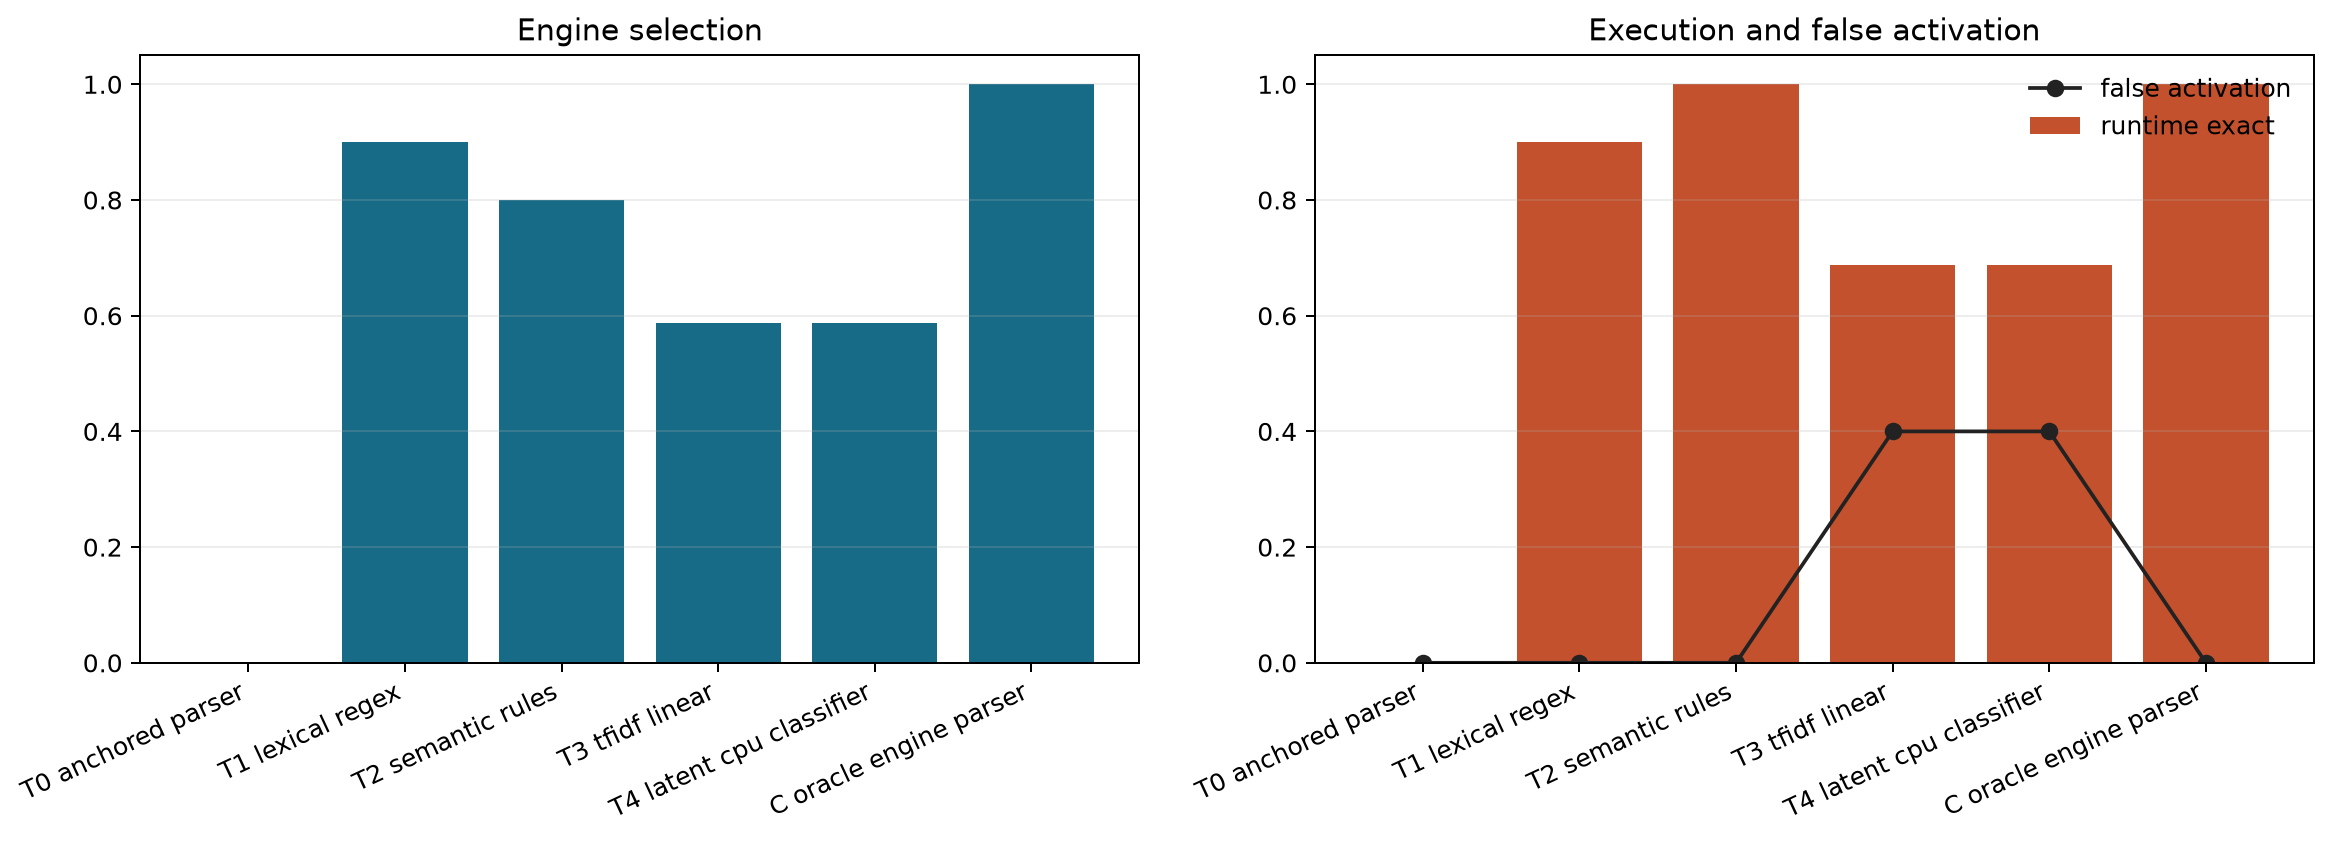
\includegraphics[width=0.92\linewidth]{paper2_trigger_ladder.png}
\caption{Six-way routing accuracy and end-to-end runtime exactness.  The oracle
parser bounds serialization; T1 is lexical and T2 exploits graph/Datalog
semantic equivalence rather than selecting every engine correctly.}
\label{fig:trigger-ladder}
\end{figure}

Shallow lexical audits do not solve the six-way task: bag-of-words, word-ngram,
character-ngram, and latent classifiers obtain 0.633, 0.593, 0.773, and 0.593
accuracy, respectively.  Their best positive engine-selection rate is 0.592.
For word TF--IDF, increasing examples per engine from 25 to 250 raises trigger
recall from 0.570 to 0.988 but also raises FAR from 0 to 0.400; selection ends at
0.588.  More rows therefore expose a decision-boundary problem rather than
repairing it.  The next justified neural experiment is factorized six-way
routing, not another joint free-form block generator.

\begin{figure}[ht]
\centering
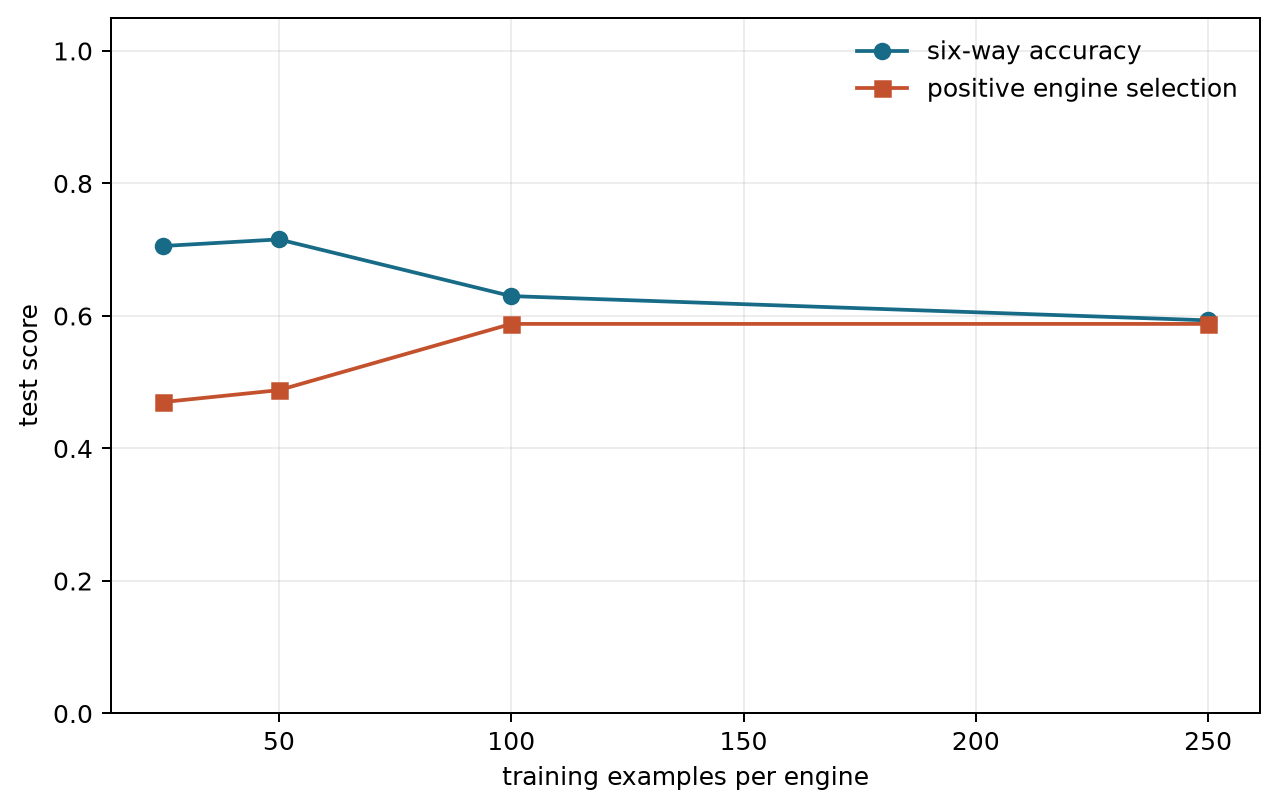
\includegraphics[width=0.78\linewidth]{paper2_diagnostic_learning_curves.png}
\caption{Word TF--IDF does not approach reliable six-way selection as the
training set grows; increasing trigger recall is accompanied by control
activation.}
\label{fig:diagnostic-learning}
\end{figure}

\subsection{Capability-count scaling and interference}

Figure~\ref{fig:scaling} and Table~\ref{tab:scaling} show that recurring context
grows with the catalog, but quality is not monotonic.  ICL is exact on all
calculator positives at one engine and all calculator/Datalog positives at two,
yet its false-activation rates are 1.0 and 0.9.  Adding graph drops positive
exactness to 0.396; at five engines exactness is 0.475 and FAR returns to 1.0.
Textual schemas always emit no execution: safe, increasingly expensive, and
inert.  Qwen weights keep a constant 26-token contract and FAR 0, but exactness
is zero at 1--3 engines and 0.188 at five because date rows enter the test mix.

\begin{figure}[ht]
\centering
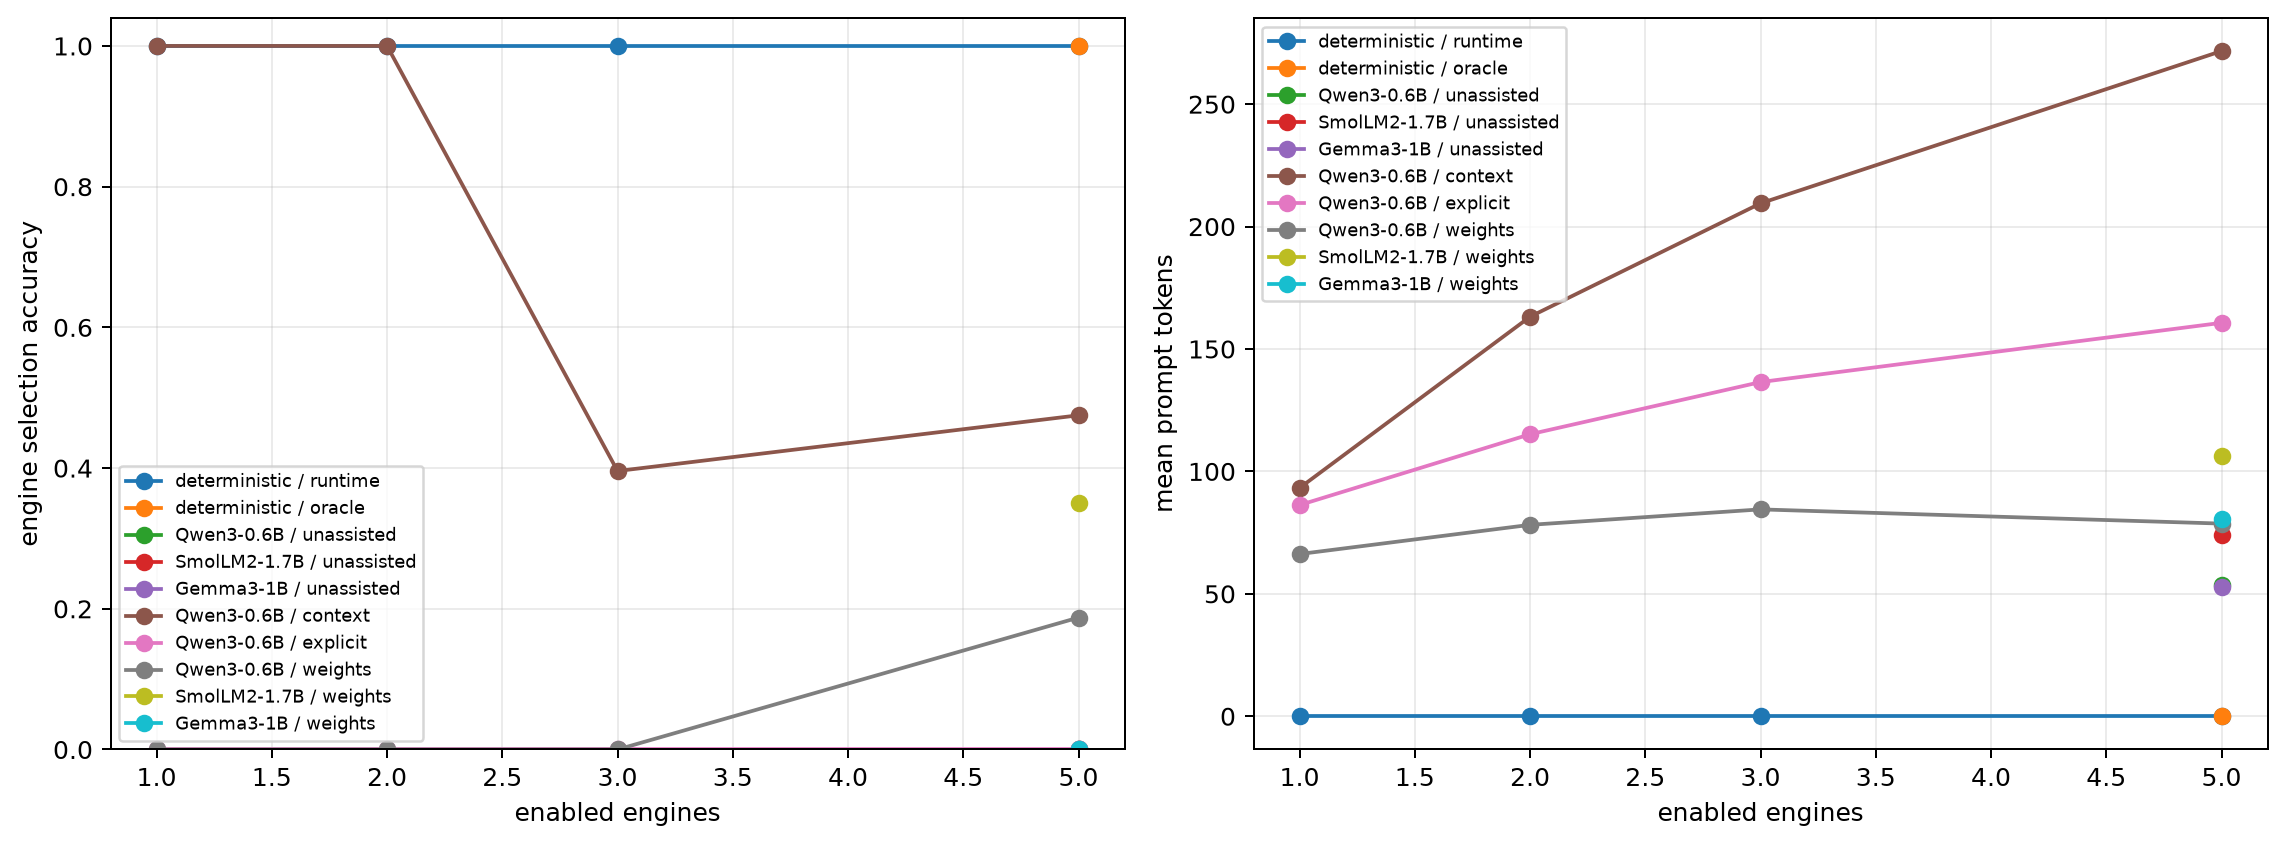
\includegraphics[width=\linewidth]{paper2_capability_scaling.png}
\caption{Engine selection and mean tokenizer prompt cost versus enabled engine
count. Deterministic and oracle lines are protocol bounds, not learned evidence.}
\label{fig:scaling}
\end{figure}

\begin{table}[ht]
\centering
\caption{Qwen capability scaling. Static is lexical interface burden; prompt is
the measured mean model-token count.}
\label{tab:scaling}
\resizebox{\linewidth}{!}{%
\begin{tabular}{lrrrrrr}
\toprule
Condition & Engines & Static & Prompt & Select/exact & FAR & Mean wall ms \\
\midrule
ICL & 1 & 39 & 93.3 & 1.000 & 1.000 & 2709 \\
ICL & 2 & 62 & 163.2 & 1.000 & 0.900 & 9846 \\
ICL & 3 & 92 & 209.5 & 0.396 & 0.200 & 4383 \\
ICL & 5 & 118 & 271.7 & 0.475 & 1.000 & 10033 \\
Text schemas & 1 & 43 & 86.3 & 0.000 & 0.000 & 705 \\
Text schemas & 2 & 56 & 115.2 & 0.000 & 0.000 & 819 \\
Text schemas & 3 & 69 & 136.5 & 0.000 & 0.000 & 957 \\
Text schemas & 5 & 95 & 160.7 & 0.000 & 0.000 & 1130 \\
Weights & 1 & 26 & 66.3 & 0.000 & 0.000 & 2479 \\
Weights & 2 & 26 & 78.2 & 0.000 & 0.000 & 6696 \\
Weights & 3 & 26 & 84.5 & 0.000 & 0.000 & 8689 \\
Weights & 5 & 26 & 78.7 & 0.188 & 0.000 & 7843 \\
\bottomrule
\end{tabular}%
}
\end{table}

\subsection{Exact execution is not exact result use}

The second model pass receives the original question and the deterministic
result, then must answer with that result only.  Qwen receives 15 such passes and
SmolLM2 receives 28.  Both have use accuracy 0.0 and override rate 1.0 among
assessed rows.  Wrong reinterpretation occurs in 11/15 Qwen passes and all 28
SmolLM2 passes.  Thus execution success is not sufficient: result preservation
is a separate failure surface that the runtime must eventually enforce.

\subsection{Typed state and bounded composition}

Forty deterministic two-stage compositions validate dependency-linked state:
20 date $\rightarrow$ calculator and 20 graph $\rightarrow$ Datalog rows.  Both
families achieve 1.0 at stage 1, stage 2, final exactness, dependency recording,
and state reuse.  Mean state sizes are 3 and 7 items, respectively.  This shows
that the typed runtime can reuse derived values without repeated model calls; it
does not show that a model can plan those compositions.

\subsection{Prototype economics}

Mean deterministic reflex wall time is below 1 ms at every catalog size on this
machine.  Model conditions range from about 0.7 s per row for an inert one-engine
schema prompt to 13.4 s for the five-engine SmolLM2 adapter.  These are
correctness-first, full-prefix prototype measurements on one Intel GPU, not
production latency estimates.  The stronger conclusion is operational: engine
CPU time is negligible relative to neural generation, but selecting and
preserving the engine result remains unreliable.

\section{Hypotheses, falsification, and gate}

\begin{itemize}
\item H1 (reliable heterogeneous learned interface) is falsified at this scale.
\item H2 (context burden grows with engine count) is supported for recurring
      tokens, but constant adapter context does not yield reliable quality.
\item H3 (assistance degrades more slowly with task difficulty) is not
      adjudicated; the frozen test varies values, not formal depth.
\item H4 (robustness to added engines) is falsified by non-monotonic ICL
      interference and learned family collapse.
\item H5 (typed-state reuse) is supported only in deterministic bounded
      compositions.
\item H6 (small-model augmentation closes a large-model gap) is not tested; no
      larger-model comparison is used to rescue a failed small-model gate.
\item H7 (deterministic serialization is the dominant failure) is falsified by
      the exact oracle-engine parser; semantic routing is the remaining upstream
      bottleneck, with result use remaining downstream.
\end{itemize}

The machine-readable gate artifact records \texttt{status: no\_go} and an empty
passing-model list.  Paper 3 may still study implicit semantic interrupts as a
new exploratory question, but this explicit multi-engine result does not justify
claiming a reliable learned predecessor.

The post-gate diagnostic does not reverse this decision.  T1 is the cheapest
passing baseline for the frozen language, but no T2--T4 semantic route clears the
selection criterion.  Consequently Paper 3 remains paused while factorized
neural routing and result-use controls are tested.

\section{Limitations}

The benchmark is synthetic and deliberately templated.  Disjoint namespaces and
a frozen test reduce leakage, but do not establish linguistic robustness.  The
runtime reflex is anchored to those templates and should not be generalized.
Only one seed, one rank, one training schedule, and three small checkpoints are
tested.  The explicit baseline uses textual schemas rather than native function
calling.  Strict exact matching penalizes semantically correct capitalization or
extra prose, appropriately for an execution protocol but more harshly than a
question-answer benchmark.  We do not add the optional sixth engine, a generic
code interpreter, an unrestricted planner, larger models, or a model-authored
composition study after the core gate fails.  Finally, measured XPU wall time is
backend- and machine-specific.

The larger diagnosis is still synthetic and has only split-level template
separation, not naturally authored language.  T1 should therefore not be read as
open-domain robustness.  Graph and Datalog deliberately share a transitive
closure subproblem; T2's runtime success shows functional substitution but also
why answer-only scoring would conceal routing errors.

A post-study TwIL-LM3/SmolLM3-3B interface pilot is retained in the repository
but excluded from the headline results.  Its Horn and graph labels were all
positive, admitting a constant-\texttt{true} neural baseline, and its
\texttt{/no\_think} 160-token budget does not match TwIL's documented
thinking-mode evaluation.  Strict rescoring does establish one useful boundary:
every exact IR executed correctly, while only 6/22 SmolLM3 and 7/22 TwIL hybrid
exact tasks had both the right formalization and result.  These are interface
diagnostics, not a ranking of internal reasoning.  A balanced, TwIL-aligned
revision is required before adding ``reasoning in weights versus coprocessors''
as a main result.

\section{Reproducibility}

The retained workflow is:

\begin{verbatim}
python -m ccpu paper2 generate-next \
  --config configs/paper2/next_iter_xpu.json \
  --output-dir artifacts/paper2/next_iter/data_v1

python -m ccpu paper2 run-next \
  --config configs/paper2/next_iter_xpu.json \
  --dataset artifacts/paper2/next_iter/data_v1/test.jsonl \
  --condition runtime --catalog-size 5 \
  --output-dir artifacts/paper2/next_iter/runtime_n5_v4

python -m ccpu paper2 analyze-next \
  --config configs/paper2/next_analysis.json \
  --output-dir artifacts/paper2/next_iter/analysis_v1

python -m ccpu paper2 generate-diagnostic \
  --config configs/paper2/diagnostic_cpu.json \
  --output-dir artifacts/paper2/diagnostic_v1/data

python -m ccpu paper2 audit-diagnostic \
  --train artifacts/paper2/diagnostic_v1/data/train.jsonl \
  --test artifacts/paper2/diagnostic_v1/data/test.jsonl \
  --output artifacts/paper2/diagnostic_v1/lexical_audit.json

python -m ccpu paper2 analyze-diagnostic \
  --train artifacts/paper2/diagnostic_v1/data/train.jsonl \
  --test artifacts/paper2/diagnostic_v1/data/test.jsonl \
  --output-dir artifacts/paper2/diagnostic_v1/analysis
\end{verbatim}

The original model runs store predictions, factorized summaries, dataset and
artifact hashes, pinned model metadata, package/device provenance, and the dirty
Git revision at execution time.  The earlier analysis artifact hashes all 22
source summaries.  The CPU diagnostic manifests record split/source hashes,
configuration, Python/platform/Git environment, predictions, and aggregate
reports.

\section{Related work}

Toolformer learns model-authored API use \cite{toolformer}; this study instead
holds execution local, typed, and fail-closed.  LoRA supplies the compact weight
placement mechanism \cite{lora}, but low adapter loss does not guarantee exact
interface generation.  AlphaGeometry combines neural guidance and symbolic
deduction in a domain-specific system \cite{alphageometry}.  Dynamic solver
composition and neurosymbolic primitive programming study richer solver
selection and composition \cite{dynamic,forethought}; our negative result is
narrower and focuses on factorized interface reliability in small models.

\section{Conclusion}

The answer to ``where should interface knowledge live?'' is asymmetric.  Exact
parsing, execution, provenance, state, and enforcement belong in the runtime.
Context can expose heterogeneous interfaces but scales in recurring tokens and
can activate when it should not.  Adapter weights keep the contract compact and
controls safe, but the tested adapters collapse across engine families and fail
to preserve exact returned values.  The missing component is therefore not
another exact engine; it is a reliable, independently validated semantic
selection and result-use policy.  Until that component clears a multi-family
held-out gate, heterogeneous learned reflex reasoning remains unconfirmed.
The larger factorization narrows the next step: keep deterministic per-engine
serialization, retain lexical routing as a bounded baseline, and train/evaluate
semantic selection independently before spending capacity on generation.

\begin{thebibliography}{9}
\bibitem{toolformer} Schick et al. Toolformer: Language Models Can Teach Themselves to Use Tools. NeurIPS, 2023.
\bibitem{lora} Hu et al. LoRA: Low-Rank Adaptation of Large Language Models. ICLR, 2022.
\bibitem{alphageometry} Trinh et al. Solving Olympiad Geometry without Human Demonstrations. Nature, 2024.
\bibitem{dynamic} Xu et al. Adaptive LLM-Symbolic Reasoning via Dynamic Logical Solver Composition. EACL, 2026.
\bibitem{forethought} Bhat et al. Forethought: Verifiable Reasoning from Neurosymbolic Primitive Programming. arXiv:2607.04096, 2026.
\end{thebibliography}

\end{document}
